\section{Meal schedule}

The two figures in this section \cref{MealScheduleList} and \cref{MealScheduleBar} displays two design ideas for the meal schedule aspect of the program.

\begin{figure}[H]
	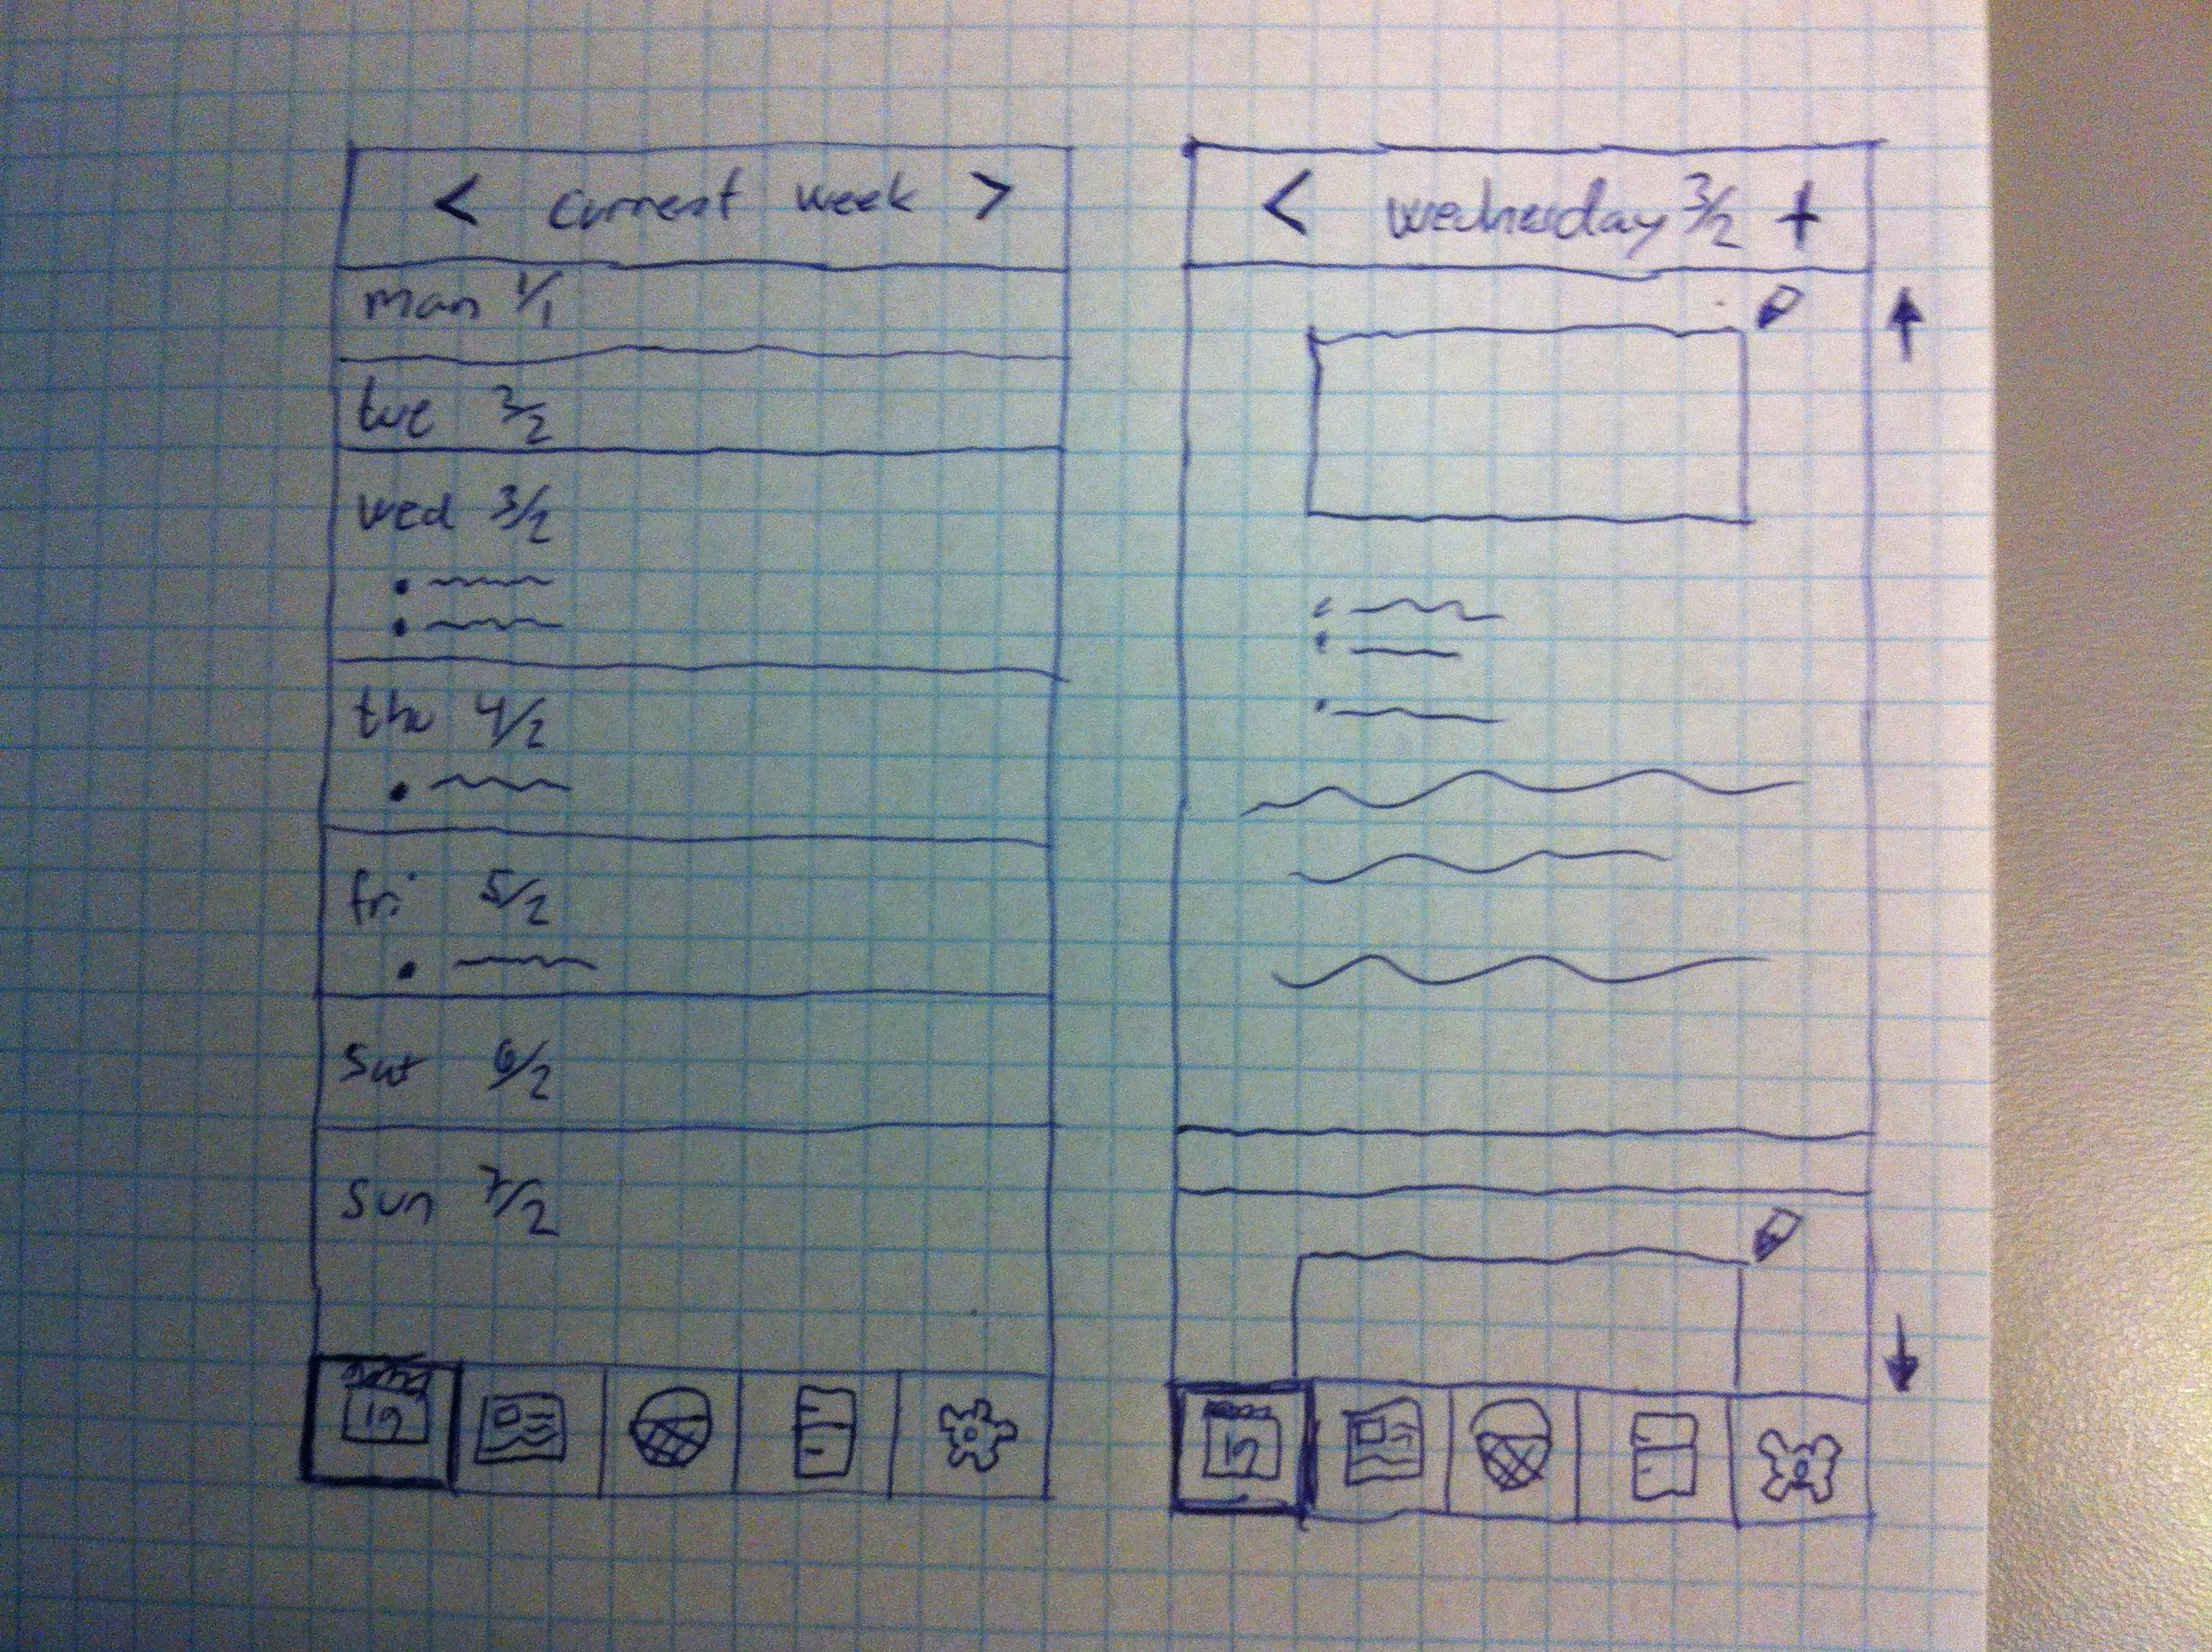
\includegraphics[width=0.8\textwidth]{Grafik/FoodPlanner/FinalMealScheduleSketch1}
	\caption{The right screen shows 7 days of a specific week and the left screen shows scheduled meals on a specific day.}
	\label{MealScheduleList}
\end{figure}

Beginning with the screen to the left on \cref{MealScheduleList} there are three areas of concern. On the bottom we have the navigation screen which is displayed throughout the program. In the middle of the screen there is a list overview of 7 days. Each day shows the names of scheduled meals on that specific day. If there are many meals scheduled the list will expand to outside of the screen view. The user can swipe to view all days and press a specific day to view details about it. This method of display gives the user an easy and informative view of the week days. 

\begin{figure}[H]
	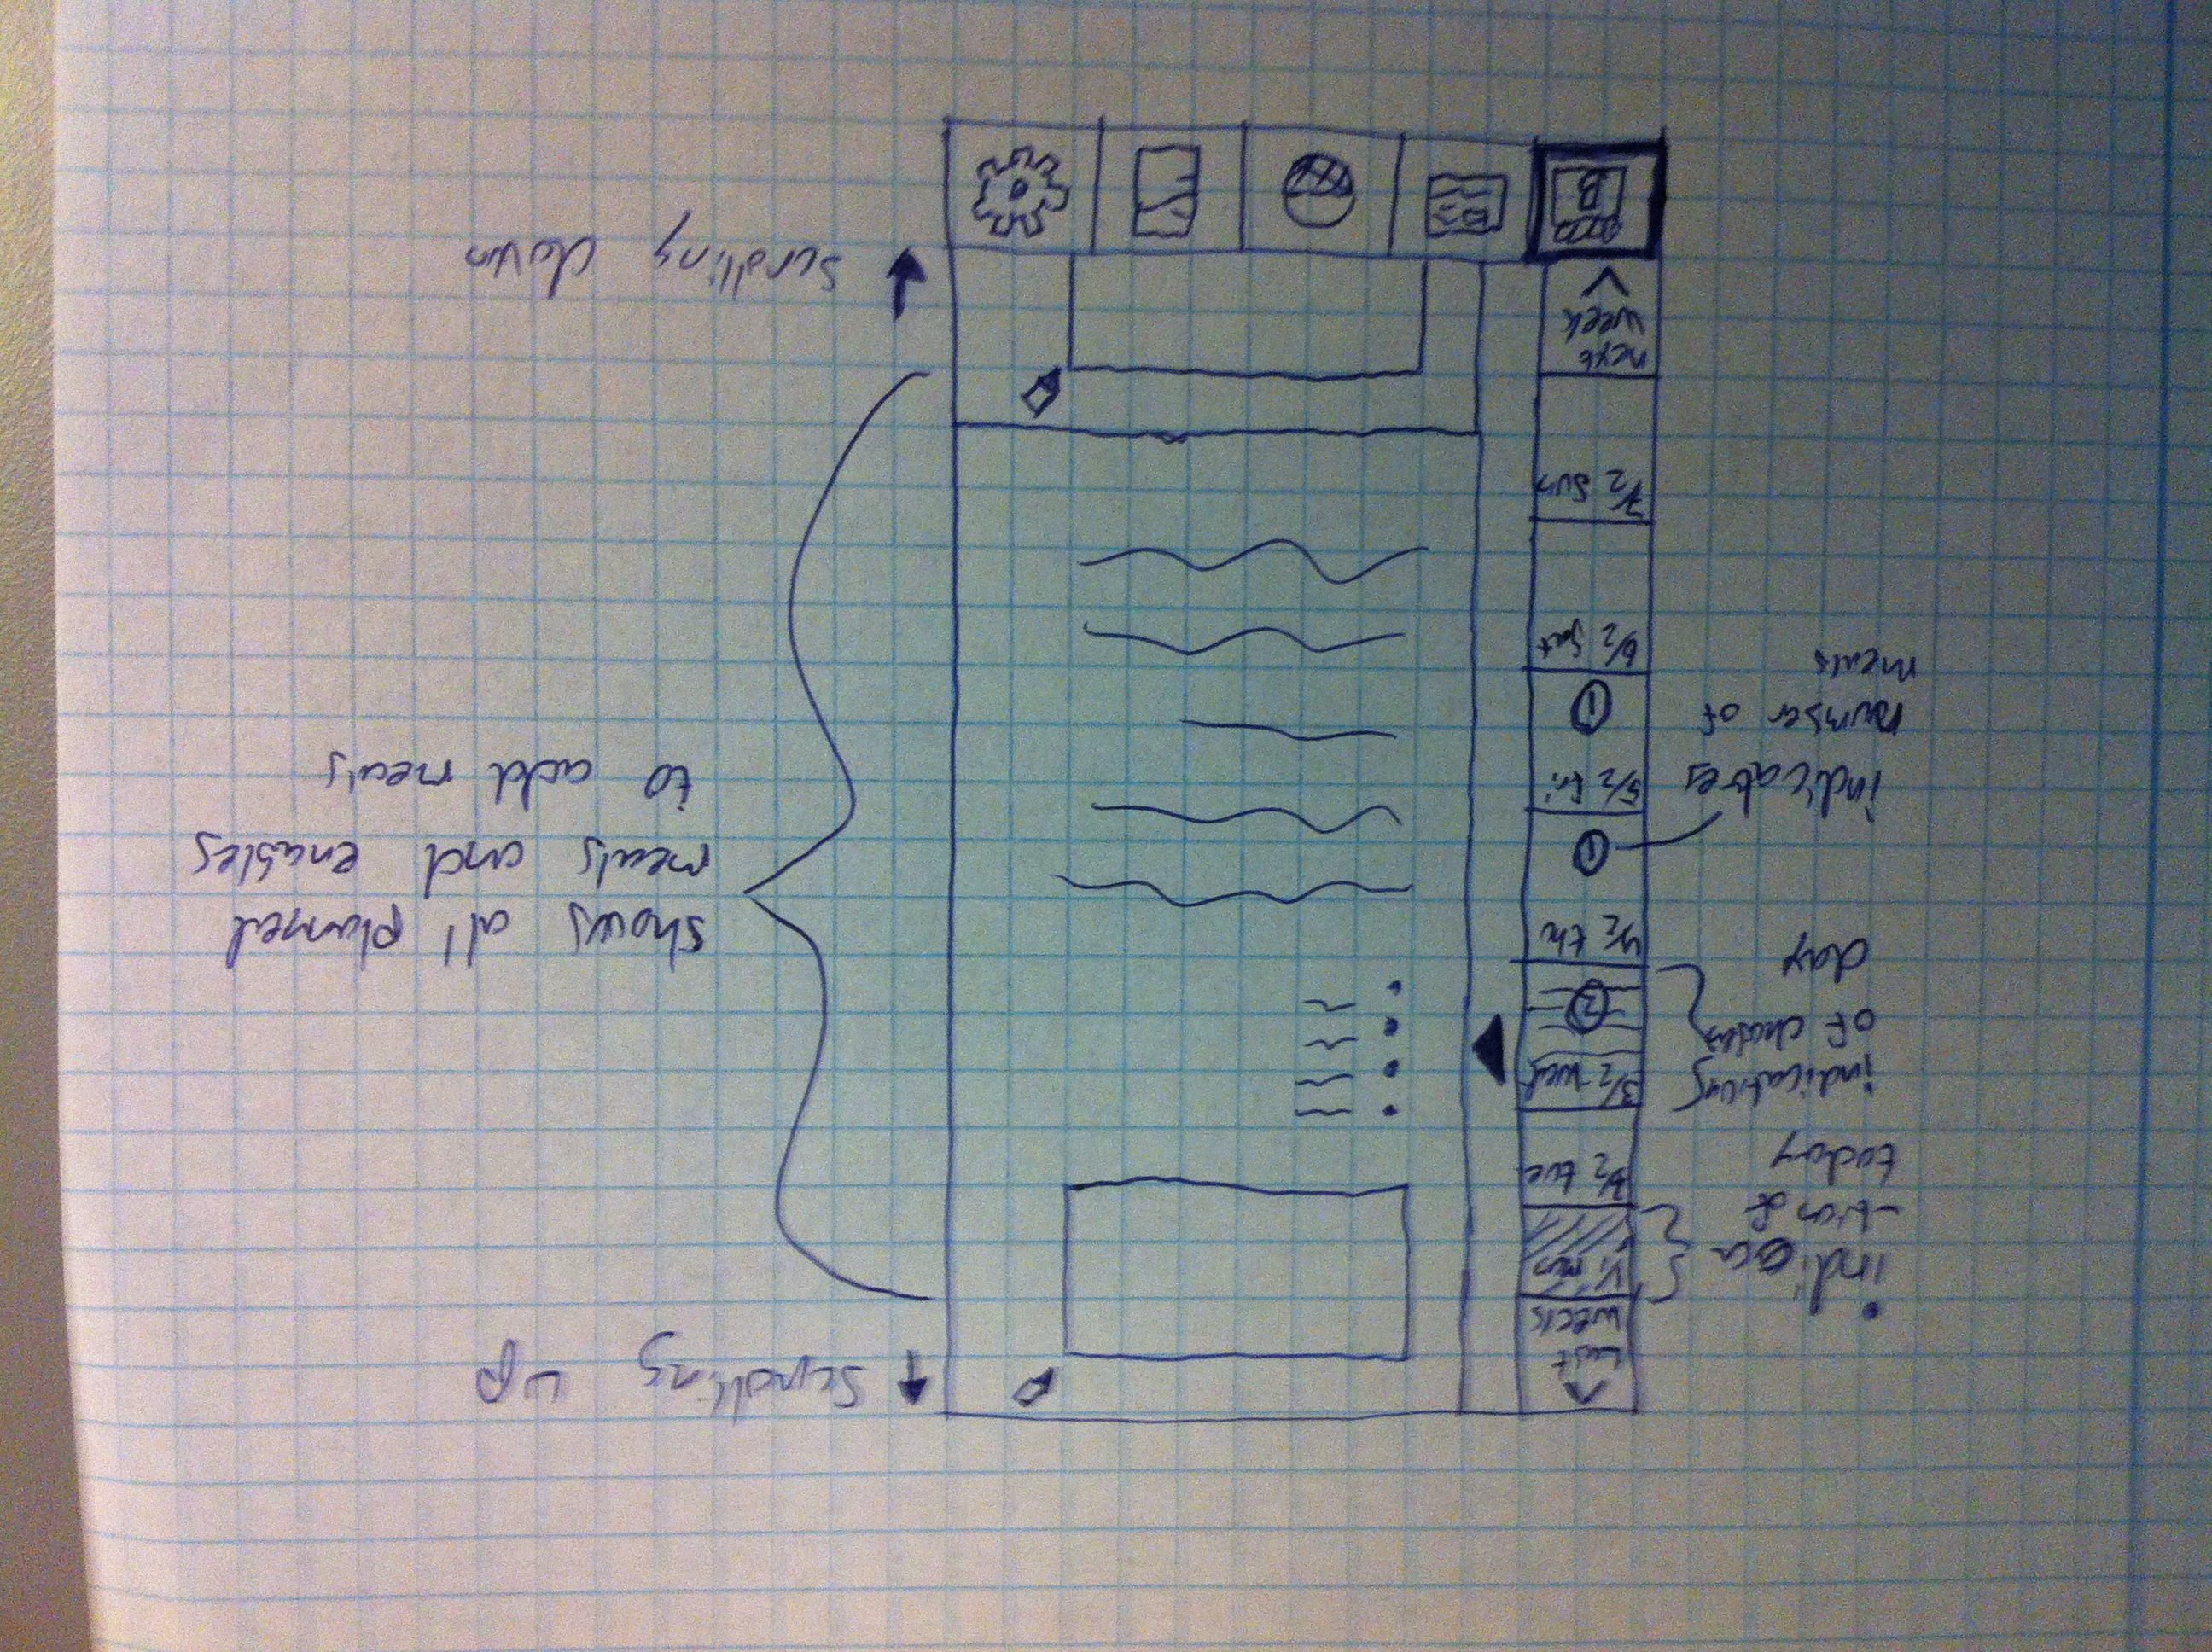
\includegraphics[width=0.8\textwidth]{Grafik/FoodPlanner/FinalMealScheduleSketch2}
	\caption{This sketch merges both of the screens above into one screen with the weeks on the left bar and the scheduled meals as a list on the right side of the screen.}
	\label{MealScheduleBar}
\end{figure}